\usepackage{pgf}
\usepackage{tikz}
\usetikzlibrary{arrows,automata,fit}

\newcommand{\ejemplografo}{
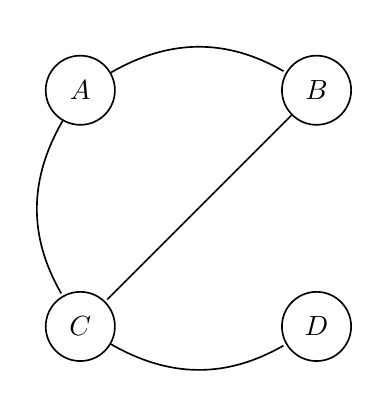
\begin{tikzpicture}[>=stealth',shorten >=1pt,auto,node distance=3cm,semithick]
  \tikzstyle{every state}=[draw=black,text=black]

  \node[state]         (A)                    {$A$};
  \node[state]         (B) [right of=A]       {$B$};
  \node[state]         (C) [below of=A]       {$C$};
  \node[state]         (D) [right of=C]       {$D$};
  
  \path (A) edge  [bend left]   node {}  (B)
            edge  [bend right]  node {}  (C)
        (B) edge                node {}  (C)
        (C) edge  [bend right]  node {}  (D);
\end{tikzpicture}}

\newcommand{\ejemplografocompleto}{
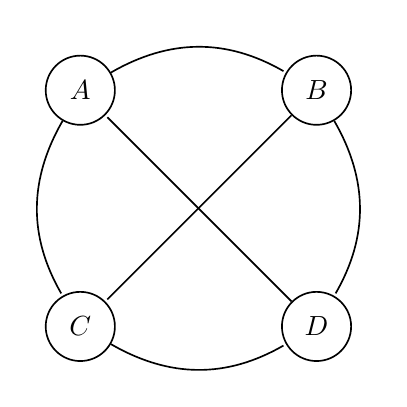
\begin{tikzpicture}[>=stealth',shorten >=1pt,auto,node distance=3cm,semithick]
  \tikzstyle{every state}=[draw=black,text=black]

  \node[state]         (A)                    {$A$};
  \node[state]         (B) [right of=A]       {$B$};
  \node[state]         (C) [below of=A]       {$C$};
  \node[state]         (D) [right of=C]       {$D$};
  
  \path (A) edge  [bend left]   node {}  (B)
            edge  [bend right]  node {}  (C)
		(B) edge  [bend left]   node {}  (D)
        (B) edge                node {}  (C)
        (D) edge                node {}  (A)
        (C) edge  [bend right]  node {}  (D);
\end{tikzpicture}}

\newcommand{\ejemplografodirigido}{
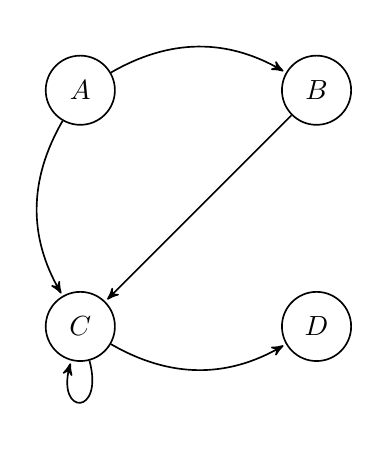
\begin{tikzpicture}[->,>=stealth',shorten >=1pt,auto,node distance=3cm,semithick]
  \tikzstyle{every state}=[draw=black,text=black]

  \node[state]         (A)                    {$A$};
  \node[state]         (B) [right of=A]       {$B$};
  \node[state]         (C) [below of=A]       {$C$};
  \node[state]         (D) [right of=C]       {$D$};
  
  \path (A) edge  [bend left]   node {}  (B)
            edge  [bend right]  node {}  (C)
        (B) edge                node {}  (C)
        (C) edge  [bend right]  node  {}  (D)
        (C) edge  [loop below]  node  {}  (C);
\end{tikzpicture}}

\newcommand{\ejemplosubgrafo}{
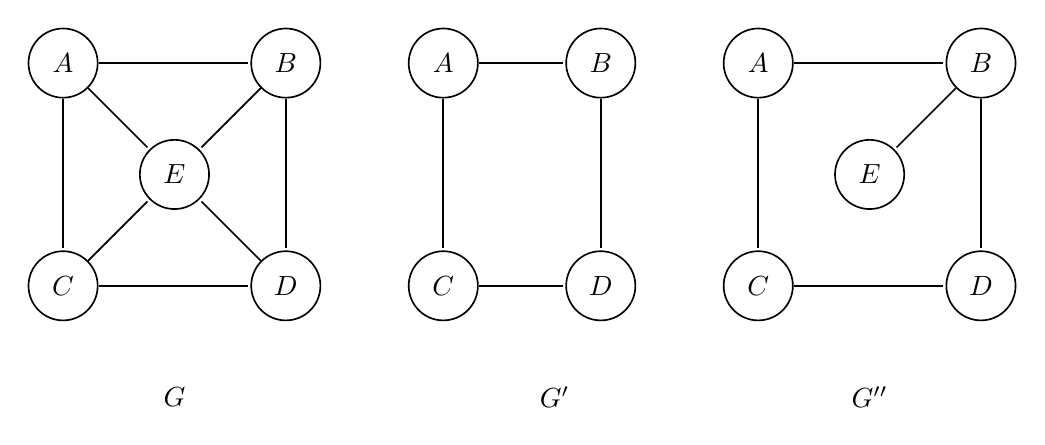
\begin{tikzpicture}[>=stealth',shorten >=1pt,auto,node distance=2cm,semithick]
  \tikzstyle{every state}=[draw=black,text=black]

% Grafo G
  \node[state]         (E)                          {$E$};
  \node[state]         (B) [above right of=E]       {$B$};
  \node[state]         (A) [above left of= E]       {$A$};
  \node[state]         (C) [below left of= E]       {$C$};
  \node[state]         (D) [below right of=E]       {$D$};

  \path (A) edge                node {}  (B)
        (A) edge                node {}  (E)
        (A) edge                node {}  (C)
        (B) edge                node {}  (D)
        (B) edge                node {}  (E)        
        (C) edge                node {}  (E)
        (C) edge                node {}  (D)
        (D) edge                node {}  (E);
        
        
% Subgrafo G'
  \node[state]         (F) [right of= B]       {$A$};
  \node[state]         (G) [right of= F]       {$B$};
  \node[state]         (H) [right of= D]       {$C$};
  \node[state]         (I) [right of= H]       {$D$};
  
  \path (F) edge                node {}  (G)
        (F) edge                node {}  (H)
        (G) edge                node {}  (I)
        (H) edge                node {}  (I);
        
% Subgrafo G'

  \node[state]         (J) [right of= G]             {$A$};
  \node[state]         (K) [right of= I]             {$C$};
  \node[state]         (N) [above right of= K]       {$E$};
  \node[state]         (M) [below right of= N]       {$D$};
  \node[state]         (L) [above right of= N]       {$B$};
  
  \path (J) edge                node {}  (K)
        (J) edge                node {}  (L)
        (L) edge                node {}  (N)
        (L) edge                node {}  (M)
        (K) edge                node {}  (M);
        
% Etiquetas con el nombre de los grafos
  \node[align=center, below right of=C] {$G$};
  \node[align=center, below right of=H] {$G'$};
  \node[align=center, below right of=K] {$G''$};
\end{tikzpicture}}

\newcommand{\ejemplounionintersecciongrafo}{
\begin{tikzpicture}[>=stealth',shorten >=1pt,auto,node distance=2cm,semithick]
  \tikzstyle{every state}=[draw=black,text=black]

% Grafo G
  \node[state]         (A)                          {$A$};
  \node[state]         (B) [below right of=A]       {$B$};
  \node[state]         (C) [below      of= B]       {$C$};
  \node[state]         (D) [right of=B]             {$D$};
  \node[state]         (E) [right of=C]             {$E$};

  \path (A) edge                node {}  (B)
        (B) edge                node {}  (C)
        (B) edge                node {}  (D)      
        (C) edge                node {}  (E)
        (D) edge                node {}  (E);
        
% Grafo G'
  \node[state]         (H) [right of= E]       {$C$};
  \node[state]         (I) [right of= D]       {$D$};
  \node[state]         (G) [right of= H]       {$E$};
  \node[state]         (F) [above right of= G] {$F$};
  
  \path (H) edge                node {}  (I)
        (I) edge                node {}  (F)
        (G) edge                node {}  (F)
        (H) edge                node {}  (G);
        
% Etiquetas con el nombre de los grafos
  \node[align=center, below right of=C] (Z) {$G$};
  \node[align=center, below right of=H] (Y) {$G'$};

% Grafo G \cup G'
  \node[state]         (J) [below left of=Z]        {$A$};
  \node[state]         (K) [below right of=J]       {$B$};
  \node[state]         (L) [below of= K]            {$C$};
  \node[state]         (M) [right of=K]             {$D$};
  \node[state]         (N) [right of=L]             {$E$};
  \node[state]         (R) [above right of=N]       {$F$};

  \path (J) edge                node {}  (K)
        (K) edge                node {}  (L)
        (K) edge                node {}  (M)      
        (L) edge                node {}  (N)
        (L) edge                node {}  (M)
        (N) edge                node {}  (R)
        (R) edge                node {}  (M)
        (M) edge                node {}  (N);
        
  \node[align=center, below right of=L] {$G \cup G'$};
  
% Grafo G \cup G'
  \node[state]         (O) [right of=R]        {$C$};
  \node[state]         (P) [right of=O]              {$E$};


  \path (O) edge                node {}  (P);
        
        
  \node[align=center, below right of=O] {$G \cap G'$};

\end{tikzpicture}}














\newcommand{\ejemplografoponderado}{
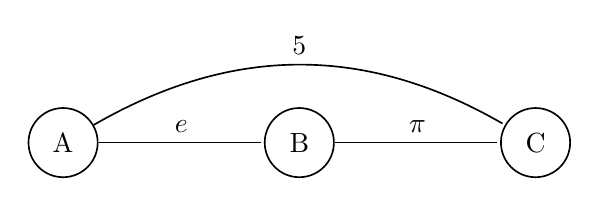
\begin{tikzpicture}[>=stealth',shorten >=1pt,auto,node distance=3cm,semithick]
  \tikzstyle{every state}=[draw=black,text=black]
 
  
  \node[state] (a)              {A};
  \node[state] (b) [right of=a] {B};
  \node[state] (c) [right of=b] {C};
  
  \path (a)     edge                node {$e$} (b);
  \path (a)   edge [bend left]   node {$5$} (c);  
  \path (b)   edge                node {$\pi$} (c);
 
  
\end{tikzpicture}}







\newcommand{\ejemplografocomplementario}{
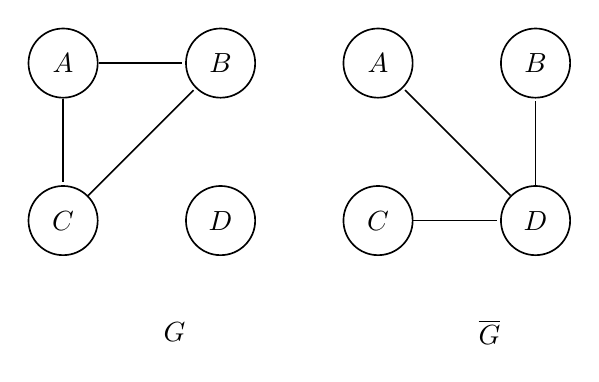
\begin{tikzpicture}[>=stealth',shorten >=1pt,auto,node distance=2cm,semithick]
  \tikzstyle{every state}=[draw=black,text=black]

% Grafo G
  \node[state]         (B)                          {$A$};
  \node[state]         (C) [below of=B]             {$C$};
  \node[state]         (D) [right of=B]             {$B$};
  \node[state]         (E) [right of=C]             {$D$};

  \path (B) edge                node {}  (C)
        (B) edge                node {}  (D)      
        (C) edge                node {}  (D);
        
% Grafo \overline{G}
  \node[state]         (H) [right of= E]       {$C$};
  \node[state]         (I) [right of= D]       {$A$};
  \node[state]         (G) [right of= H]       {$D$};
  \node[state]         (F) [right of= I]       {$B$};
  
  \path (G) edge                node {}  (I)
        (G) edge                node {}  (F)
        (H) edge                node {}  (G);
        
% Etiquetas con el nombre de los grafos
  \node[align=center, below right of=C] (Z) {$G$};
  \node[align=center, below right of=H] (Y) {$\overline{G}$};


\end{tikzpicture}}

\newcommand{\ejemplografodominancia}{
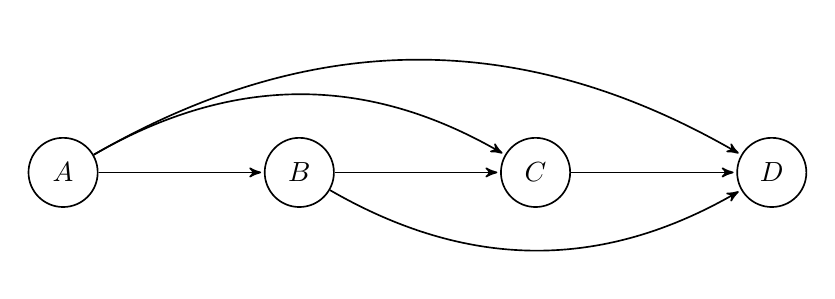
\begin{tikzpicture}[->,>=stealth',shorten >=1pt,auto,node distance=3cm,semithick]
  \tikzstyle{every state}=[draw=black,text=black]
 
  
  \node[state] (A)              {$A$};
  \node[state] (B) [right of=A] {$B$};
  \node[state] (C) [right of=B] {$C$};
  \node[state] (D) [right of=C] {$D$};
  
  \path (A) edge              node {} (B);
  \path (A) edge [bend left]  node {} (C);
  \path (A) edge [bend left]  node {} (D);
  \path (B) edge              node {} (C);
  \path (B) edge [bend right] node {} (D);
  \path (C) edge              node {} (D);
  
\end{tikzpicture}}

\newcommand{\ejemplografocompetitividad}{
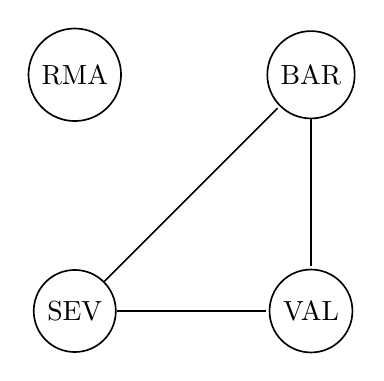
\begin{tikzpicture}[>=stealth',shorten >=1pt,auto,node distance=3cm,semithick]
  \tikzstyle{every state}=[draw=black,text=black]
 
  \node[state] (RMA)                      {RMA};
  \node[state] (BAR) [right       of=RMA] {BAR};
  \node[state] (SEV) [below       of=RMA] {SEV};
  \node[state] (VAL) [below       of=BAR] {VAL};
  
  \path (SEV)   edge                node {} (BAR);
  \path (SEV)   edge                node {} (VAL);  
  \path (BAR)   edge                node {} (VAL);
  
\end{tikzpicture}}

\newcommand{\ejemplografocompetitividadevolutivo}{
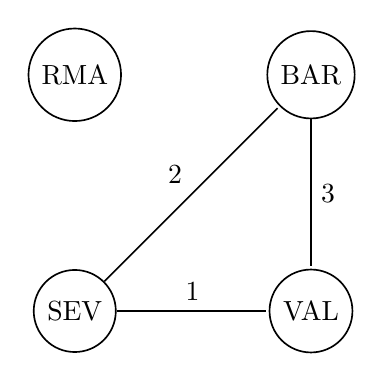
\begin{tikzpicture}[>=stealth',shorten >=1pt,auto,node distance=3cm,semithick]
  \tikzstyle{every state}=[draw=black,text=black]
 
  \node[state] (RMA)                      {RMA};
  \node[state] (BAR) [right       of=RMA] {BAR};
  \node[state] (SEV) [below       of=RMA] {SEV};
  \node[state] (VAL) [below       of=BAR] {VAL};
  
  \path (SEV)   edge                node {2} (BAR);
  \path (SEV)   edge                node {1} (VAL);  
  \path (BAR)   edge                node {3} (VAL);
  
\end{tikzpicture}}


\newcommand{\ejemplogradomedio}{
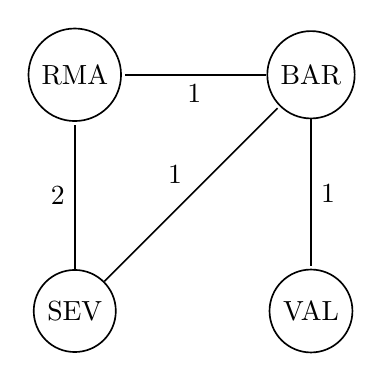
\begin{tikzpicture}[>=stealth',shorten >=1pt,auto,node distance=3cm,semithick]
  \tikzstyle{every state}=[draw=black,text=black]
 
  \node[state] (RMA)                      {RMA};
  \node[state] (BAR) [right       of=RMA] {BAR};
  \node[state] (SEV) [below       of=RMA] {SEV};
  \node[state] (VAL) [below       of=BAR] {VAL};
  
  \path (SEV)   edge                node {1} (BAR);
  \path (SEV)   edge                node {2} (RMA);  
  \path (BAR)   edge                node {1} (VAL);
  \path (BAR)   edge                node {1} (RMA);
  
\end{tikzpicture}}